\documentclass[11pt]{article}

\author{Darren Hushak}
\title{CPRE 310 - Page Rank Project}
\date{\today}

\usepackage{amsmath}
\usepackage{hyperref}
\usepackage{tikz}
\usepackage{multicol}
\usepackage{color}
\usepackage{hyperref}
	\hypersetup{colorlinks}
	\hypersetup{linkcolor=blue}
	
\usetikzlibrary{arrows}
\newcommand{\cmd}[1]{\texttt{#1}}
\usepackage{listings}
\lstset{ %
language=java,                % choose the language of the code
basicstyle=\footnotesize,       % the size of the fonts that are used for the code
numbers=left,                   % where to put the line-numbers
numberstyle=\footnotesize,      % the size of the fonts that are used for the line-numbers
stepnumber=1,                   % the step between two line-numbers. If it is 1 each line will be numbered
numbersep=5pt,                  % how far the line-numbers are from the code
backgroundcolor=\color{white},  % choose the background color. You must add \usepackage{color}
showspaces=false,               % show spaces adding particular underscores
showstringspaces=false,         % underline spaces within strings
showtabs=false,                 % show tabs within strings adding particular underscores
frame=single,           % adds a frame around the code
tabsize=2,          % sets default tabsize to 2 spaces
captionpos=b,           % sets the caption-position to bottom
breaklines=true,        % sets automatic line breaking
breakatwhitespace=false,    % sets if automatic breaks should only happen at whitespace
escapeinside={\%*}{*)}          % if you want to add a comment within your code
}


\begin{document}
\maketitle
\section*{Overview}
This project was an implementation of two separate algorithms to determine ranking of a web page based on the "Page Rank" algorithm originally developed by Larry Page, CEO of Google. The project is written in Java, and accepts as input a text file representing a set of hyperlinks between webpages. The two algorithms implemented in this project are called the \hyperref[sec:power]{Power Iteration} method and the \hyperref[sec:monte]{Monte Carlo method}. These algorithms and their implementation will be detailed shortly.

\section*{The Page Rank Heuristic}
Essentially, Page Rank is an heuristic to determine a so-called "importance" of a webpage. The quantitative measurement of importance is calculated from the incoming hyperlinks to said webpage, weighted by the rank of the referring page. In short, the more incoming links a page has, the more important it is. The compelling portion of the heuristic comes from the fact that pages of higher importance pointing to another page will increase the referred page's importance even more.
\newline

\section*{Modeling Web Pages and Links}
A graph theory reduction is generally the simplest way to approach this problem. Assume a directed graph, whose vertices are individual webpages, and whose directed edges are hyperlinks from one webpage to another webpage. We can then use graph traversal algorithms to calculate page rank for each node.
\newline

For instance, the code for the two webpages on the left can be represented by this simple graph on the right:
\begin{multicols}{2}
1.html:
\begin{verbatim}
<html>
    <body>
        <a href="2.html">
        Link to 2</a>
    </body>
</html>

\end{verbatim}


2.html:
\begin{verbatim}
<html>
    <body>
        No links!
    </body>
</html>
\end{verbatim}
\columnbreak
\begin{center}
\label{fig:webgraph}
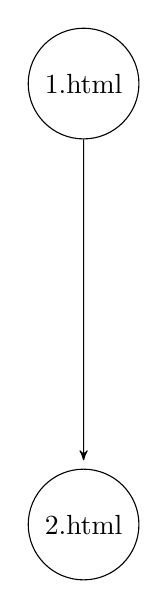
\begin{tikzpicture}
  [->,>=stealth',shorten >=3pt, scale=.8,auto=left,every node/.style={circle, minimum width=40pt, draw}]
  \node (n1) at (5,10) {1.html};
  \node (n2) at (5,3)  {2.html};

  \foreach \from/\to in {n1/n2}
    \draw (\from) -> (\to);

\end{tikzpicture}
\end{center}
\end{multicols}

Every outgoing link from a webpage will represent another directed edge from that webpage's node to the node of the webpage that that link is pointing to.
\newline

Note that in all of these calculations, self referencing edges (links within a page to itself) and duplicate edges (multiple links from one page to another) are ignored.

\section*{Model Implementation}
In my implementation, I chose to use a list of nodes (\verb!PageNode.java!) to represent all of the webpages, and a two-dimensional array as an adjacency matrix to represent all the links (\verb!LinkTable.java!).
\newline

The \verb!PageNode! class is simply a container for an \verb!int! index and a \verb!float! Page Rank. Its methods are as follows:
\begin{itemize}
\item \verb!boolean UpdatePageRank(float newPageRank, float iterThreshold)! - if \verb!pageRank - newPageRank < iterThreshold!, then this method returns \verb!false!, else it updates the \verb!pageRank! with \verb!newPageRank! and returns \verb!true!
\item \verb!float getPageRank()! - Returns the \verb!PageRank!
\item \verb!getIndex()! - Returns the integer \verb!index! of that page
\end{itemize}

The \verb!LinkTable! class contains a two-dimensional array representing an adjacency matrix of the pages. I chose a simple \verb!int[numPages][numPages]! array to keep accesses and references quick and easy. It also made determination of outdegree and indegree simple, as each is simply a sum of the row \verb!table[pageIndex][...]!, or sum of the column \verb!table[...][pageIndex]!, respectively.
The \verb!LinkTable! methods are as follows:
\begin{itemize}
\item \verb!void addLink(int fromIndex, int toIndex)! - Sets the value at location \verb![fromIndex][toIndex]! to 1, to represent a link
\item \verb!int getLinks(int fromIndex, int toIndex)! - Returns the value at \verb![fromIndex][toIndex]!
\item \verb!int getTotalOutboundLinks(int fromIndex)! - Returns the outdegree of the page with index \verb!fromIndex!
\item \verb!int getTotalInboundLinks(int toIndex)! - Returns the indegree of the page with index \verb!toIndex!
\item \verb!float getTotalInboundLinkShare(int fromIndex, int toIndex)! - Returns the \hyperref[eq:poweriter]{$\frac{|E(j,i)|}{deg^+V(j)}$} portion of the \hyperref[sec:power]{Power Iteration Algorithm}
\item \verb!int getRandomLink(int index)! - returns an index of a random page to jump to (there must exist a link from \verb!index! to the returned index) - necessary for the \hyperref[sec:monte]{Monte Carlo Algorithm}
\end{itemize}

To generate the model, the \verb!PageRank! class accepts two arguments: an input file name (\verb!inFile!), and an integer value of the total number of pages (\verb!numPages!) represented in the input file.

\verb!inFile! contains pairs of numbers representing a link from one page to another. This can be interpreted two ways. 
First, the first number is the source page, and the second number is the destination page: \verb!1 2! for the \hyperref[fig:webgraph]{example} given previously.
Second, the source and destination could be swapped: \verb!2 1! for the \hyperref[fig:webgraph]{example} given previously.

The \verb!PageRank! class starts by creating an array of pages of size equal to \verb!numPages!, assigning an incrementing index to each generated \verb!PageNode!. It then parses through \verb!inFile! line by line, and adds a link to the \verb!LinkTable! for each pair of numbers given. Note that \verb!PageRank! does this setup twice: once for the source $\to$ destination interpretation of the input file, and once for the destination $\to$ source interpretation. It then runs both algorithms on each interpretation.

\section*{Page Rank Algorithm: Power Iteration Method}
\label{sec:power}
This algorithm uses an iterative method to traverse every node in the graph, continually updating each page's page rank upon each iteration. The iteration ceases once a certain "iteration threshold" has been reached. This threshold is the largest change in page rank allowable to continue iteration. Therefore, upon completing an iteration in which the page rank of each node changes by less than the threshold, the algorithm is complete.
\newline

Before beginning the algorithm, every page's Page Rank is set to zero: $\forall i \in G, P(i) = 0.0$. Then, for each iteration, the page rank $P(i)$ of page $i \in G$ is calculated using the following formula:
\label{eq:poweriter}
\[
P(i) = (1 - d) + d *\left[ \sum_{j=1}^{n} \left(\frac{P(j) * |E(j,i)|}{deg^+V(j)}\right) \right]
\]

Where:
\begin{itemize}
\item $n$ is the total number of pages
\item $P(a)$ is the Page Rank of a given page $a$
\item $0 < d < 1$ is termed the "Damping Factor," and is set by the user 
\item $|E(j,i)|$ is the total number of edges from page $j$ to page $i$; if there is no edge, this equals $0$ and page $j$ contributes nothing to the Page Rank of $j$
\item $deg^+V(j)$ is the outdegree (total number of outgoing edges) of the vertex representing page $j$
\end{itemize}

Again, this equation represents a calculation done once per iteration $k$ through the Power Iteration algorithm. Once $\forall i \in G, P(i)_{k-1} - P(i)_k < threshold$, the algorithm is complete.
\newline

Upon completion, the algorithm will output a set of page ranks for each page, higher ranks indicating more importance. In general, the page ranks distribute themselves relatively close to 1.0, with a small amount of outliers.

\section*{Power Iteration Implementation}
The power iteration implementation was pretty straightforward, once the methods of the associated modeled subclasses had been laid out and implemented. Here is the code for the \verb!calculatePowerIteration! method, which returns the total number of iterations:
\begin{lstlisting}
public int calculatePowerIteration(float iterLimit) {
		boolean continueIteration = true;
		float newRankSum;
		int iterCntr = 0;
		// Check if we've reached the iteration Limit
		while (continueIteration) {
			continueIteration = false;
			// Update the pagerank of every page
			for (int i = 0; i < pageList.length; i++) {
				newRankSum = 0;
				// Sum the page rank share of each incoming page
				for (int j = 0; j < pageList.length; j++) {
					// PageRank(j) * deg+(j)
					newRankSum += pageList[j].getPageRank()
							* table.getTotalInboundLinkShare(j, i);
				}
				// Apply Damping factor
				newRankSum *= dampingFactor;
				// Add 1 - damping factor
				newRankSum += (1 - dampingFactor);
				// Update the page rank and OR= with the continue
				// Iteration checker to see if we need to continue
				// Note that if any of the pageRank updates are greater than the
				// iterLimit, continueIteration will be true for the rest of
				// this iteration, thus calling another one
				continueIteration |= pageList[i].UpdatePageRank(newRankSum,
						iterLimit);
			}
			iterCntr++;
		}
		return iterCntr;
	}
\end{lstlisting}

\section*{Page Rank Algorithm: Monte Carlo Method}
\label{sec:monte}
The second method of Page Rank determination takes a different approach to the same model of "more links $\implies$ more importance." Instead of iteratively counting links inward to pages from other pages, the Monte Carlo method models the traversal as a "random walk," where a "casual surfer" will start at a randomly selected node $i$, and with probability $\alpha$ will take a path along edge $E(i,j\in N_G(i)$, where $j$ is an edge randomly selected from the set of all neighboring edges of $i$, $N_G(i)$. Each edge $E(i,j\in N_G(i))$ has an equal probability of being selected.

This casual surfer will continue to take paths along these outgoing edges with probability $\alpha$ for a number of iterations. As soon as the random selection selects not to continue, that iteration ends. The Monte Carlo method then counts which page each of these iteration ends on for a certain number of "walks" $N$ for each node $i\in G$. It will then divide these counts by the total number of walks times the number of nodes $N * |V \in G|$ to give a normalized probability of landing on each page. These normalized probabilities (theoretically taken as $\lim_{N \to \infty}$) represent the page rank for each page.

Note that the final numbers of the page rank for the Monte Carlo method are not easily comparable to that of the Power Iteration. The Monte Carlo method gives a discrete probability distribution, the sum of each rank equaling one, whereas the Power Iteration gives page ranks roughly centered around 1, the sum of all is close to the number of nodes.

\section*{Monte Carlo Implementation}
Again, once the methods for all of the graph models were implemented, the Monte Carlo implementation was relatively straightforward:
\begin{lstlisting}
public float calculateMonteCarlo(int numRuns, float alpha) {
		// Array of hits to count for each page
		float hits[];
		hits = new float[pageList.length];
		// Sum of probability of all hits
		float totalHits = 0;
		// Random number generator
		Random rand = new Random();
		// The current page location of our "random surfer"
		int currentPageIndex;

		// For each page...
		for (int i = 0; i < pageList.length; i++) {
			// Start on a page
			currentPageIndex = i;
			// Run numRuns times...
			for (int j = 0; j < numRuns; j++) {
				// Randomly determine whether or not to stop
				while (rand.nextFloat() < alpha) {
					// If not stopping, Randomly jump to another page
					currentPageIndex = table.getRandomLink(currentPageIndex);
				}
				// Increment the counter for this page because we've stopped
				// here
				hits[currentPageIndex]++;
			}
		}
		// For each page...
		for (int i = 0; i < pageList.length; i++) {
			// Divide the number of hits by the total number of runs
			// (normalizing all of the probabilities)
			hits[i] /= (float) pageList.length * numRuns;
			totalHits += hits[i];
			// Uptate all of the pageNodes pagerank
			pageList[i].UpdatePageRank(hits[i], 0);
		}
		// Return the sum of all probabilities of arriving on a page (should
		// equal very close to 1)
		return totalHits;
	}
\end{lstlisting}
\section*{Closing Summary}
This project was a good exploration of various implementations and interpretations of the Page Rank problem. I learned a lot about the problem itself, as well as expanded my capacity for abstract thought, namely the ability to model a complex real world application such as this as a simple graph model. Once in the graph model, traversal, calculation, and other implementations were quite straightforward, leading to a nice and clean set of code producing page ranks for a number of webpage link configurations.

\newpage
\section*{Use}
To make: 

	\verb!$ make!
\newline

To run:
	Place page link input file in the same directory as the made class files. 
	If it's in the wrong directory, it will tell you where to put it.
	
	\verb!$ java PageRank <inputFile.txt> <numberOfPages>!
	\newline
	
Output:
	
	The PageRank program will print out sets of page ranks (each separated by an empty line) for the pages using the
	following algorithms:
	\begin{itemize}
	\item  Power Iteration, interpreting the input file as "SRC linksTo DST"
	\item Monte Carlo, interpreting the input file as "SRC linksTo DST"
	\item Power Iteration, interpreting the input file as "DST linksFrom SRC"
	\item Monte Carlo, interpreting the input file as "DST linksFrom SRC"
	\end{itemize}

\end{document}

